\chapter{LC-MS/MS}\label{appSec:LCMS}

\begin{table}
\centering
\caption{Gradient between the two mobile phases used during UPLC-MS/MS. Water phase (A): Milli-Q water with 2 mM ammonium acetate, organic phase (B): pure MeOH. Run time = 6 min.}
\label{apptab:gradient}
\begin{tabular}{ccccc} \toprule
\multicolumn{1}{l}{\textbf{Time (min)}} & \multicolumn{1}{l}{\textbf{Flow}} & \multicolumn{1}{l}{\textbf{\% A}} & \multicolumn{1}{l}{\textbf{\% B}} & \multicolumn{1}{l}{\textbf{Step}} \\ \midrule
0 & 0.25 & 80 & 20 & Init \\
0.1 & 0.25 & 80 & 20 & 6 \\
0.2 & 0.25 & 50 & 50 & 6 \\
0.8 & 0.25 & 30 & 70 & 6 \\
1.5 & 0.25 & 20 & 80 & 6 \\
2.8 & 0.25 & 15 & 85 & 5 \\
4.5 & 0.25 & 0 & 100 & 6 \\
5.5 & 0.25 & 0 & 100 & 6 \\
5.6 & 0.25 & 80 & 20 & 6 \\
6 & 0.25 & 80 & 20 & 6 \\ \bottomrule
\end{tabular}
\end{table}

\begin{table}
\centering
\caption{Tune parameters for UPLC-Xevo TQS instrument.}
\label{apptab:tune}
\begin{tabular}{ll} \toprule
\multicolumn{1}{c}{\textbf{ESI (-)}} &  \\ \midrule
Capillary (kV) & 2 \\
Cone (V) & 25 \\
Source Offset (V) & 40 \\
Desolvation temperature   (\textdegree C) & 450 \\
Desolvation Gas flow   (L/h) & 650 \\
Cone (L/h) & 150 \\
Nebuliszer (Bar) & 6 \\
Source Temperature (\textdegree C) & 150 \\ \bottomrule
\end{tabular}
\end{table}

\begin{figure}
    \centering
    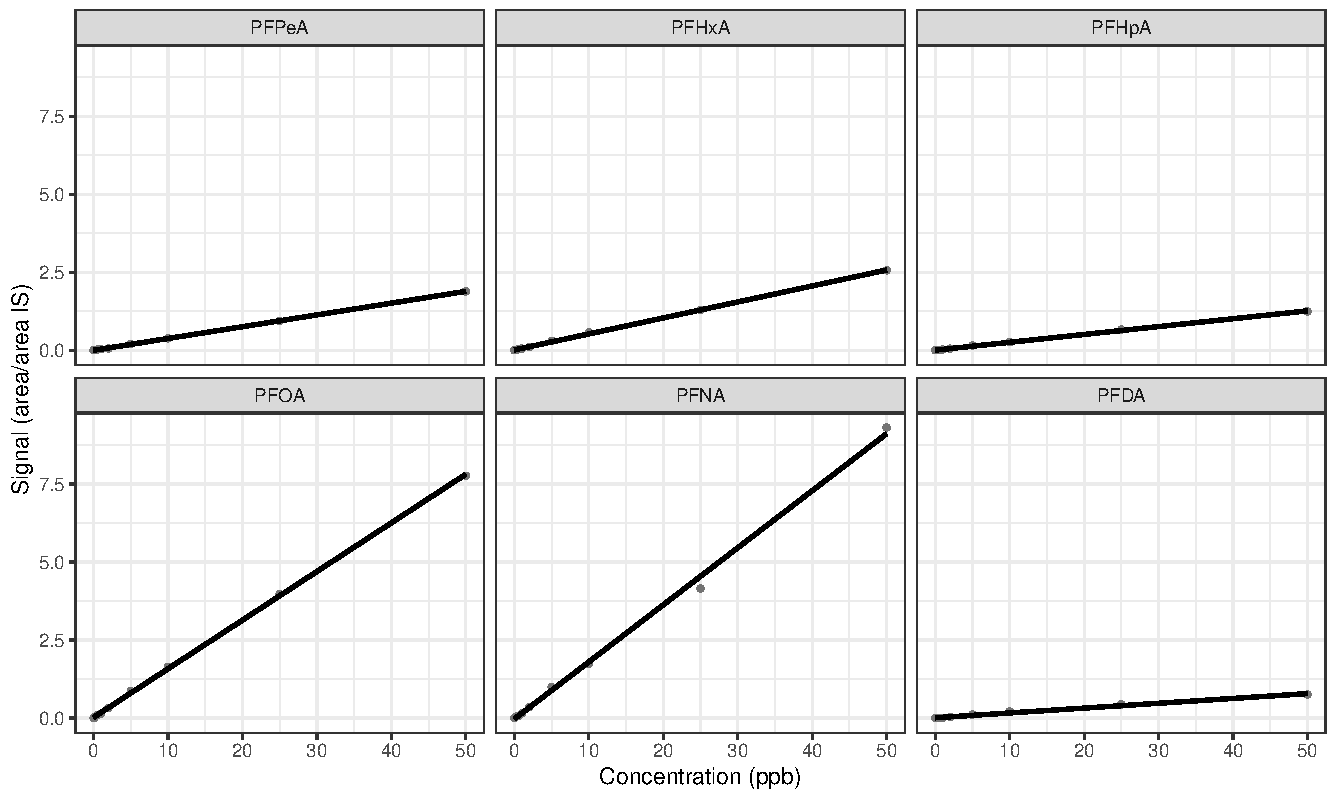
\includegraphics[width=\textwidth]{R/figs/CC_all.pdf}
    \caption{Calibration curve solvent blank}
    \label{appfig:CC}
\end{figure}

Matrix effect

\begin{figure}
    \centering
    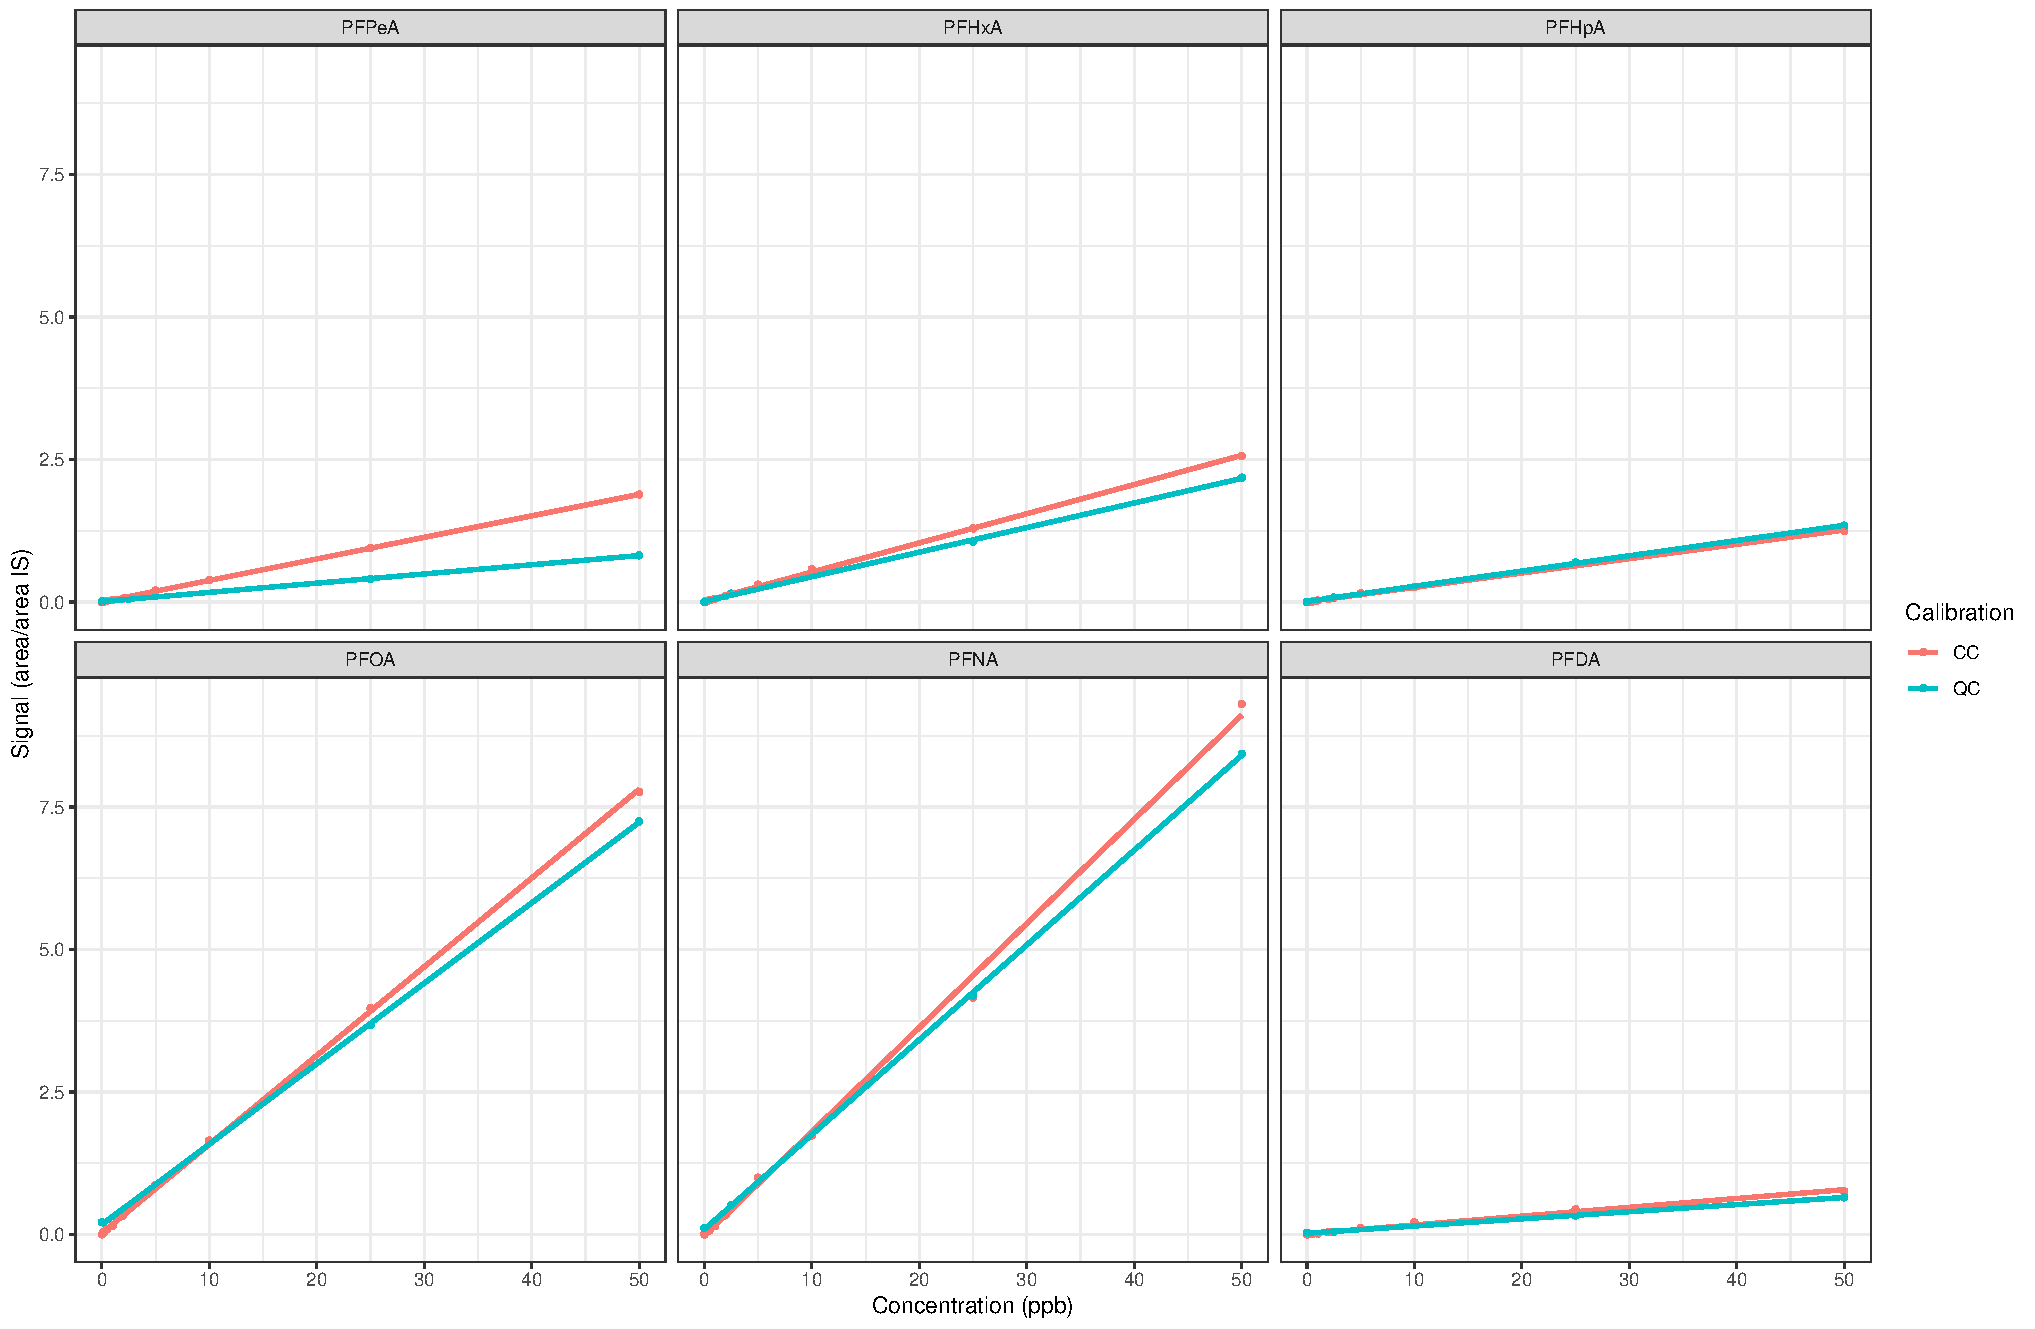
\includegraphics[width=\textwidth]{R/figs/CCQC_matrixeffect.pdf}
    \caption{Matrix effect (ME) for the PFCAs where CC = calibration curve in solvent blank, QC = matrix matched calibration curve. QC in line with CC indicates no ME, QC \textgreater CC = ion enhancement, CC \textless QC = ion suppression.}
    \label{appfig:ME}
\end{figure}